\chapter{\IfLanguageName{dutch}{Stand van zaken}{State of the art}}%
\label{ch:stand-van-zaken}

% Tip: Begin elk hoofdstuk met een paragraaf inleiding die beschrijft hoe
% dit hoofdstuk past binnen het geheel van de bachelorproef. Geef in het
% bijzonder aan wat de link is met het vorige en volgende hoofdstuk.

% Pas na deze inleidende paragraaf komt de eerste sectiehoofding.
% Voor literatuurverwijzingen zijn er twee belangrijke commando's:
% \autocite{KEY} => (Auteur, jaartal) Gebruik dit als de naam van de auteur
%   geen onderdeel is van de zin.
% \textcite{KEY} => Auteur (jaartal)  Gebruik dit als de auteursnaam wel een
%   functie heeft in de zin (bv. ``Uit onderzoek door Doll \& Hill (1954) bleek
%   ...'')

In deze stand van zaken zal worden besproken welke gassen er voorkomen in een stalomgeving en welke concentraties schadelijk zijn voor dieren en mensen. Hierna zal er worden gekeken naar welke soorten gassensoren er bestaan en hoe deze te werk gaan. Vervolgens wordt er gefocust op de MQ-sensor, door middel van sectie~\ref{sec:welke-stalgassen} wordt nagegaan welke MQ-sensoren het meest geschikt zijn om de meest voorkomende stalgassen te meten. Vervolgens wordt besproken hoe er nauwkeurigere resultaten kunnen worden bekomen, door middel van een implementatie van een warmte-koelcyclus en een DHT22 sensor.


\section{Welke gassen komen voor in stalomgevingen}%
\label{sec:welke-stalgassen}

Varkensmest bestaat voor het grootste deel uit afvalstoffen, bacteriën en eiwitten. Stalgassen ontstaan doordat andere bacteriën deze eiwitten afbreken tot giftige gassen \autocite{Wolf2013}. Deze gassen worden dus voortdurend gemaakt maar kunnen in grote hoeveelheden voorkomen als de mest in beweging komt of als er voer in de mestput gemorst wordt \autocite{Wolf2013}. Wanneer er niet genoeg ventilatie is kan dit zeer gevaarlijk zijn \autocite{Heesbeen2021}. Volgens \textcite{Klooster1993} zijn de meest voorkomende stalgassen in een varkensstal ammoniak (NH\textsubscript{3}) en koolstofdioxide (CO\textsubscript{2}), maar gassen zoals methaan (CH\textsubscript{4}), koolstofmonoxide (CO) en ammonium (NH\textsubscript{4}) behoren ook tot de vaste bewoners van de veestal.

Ammoniak is een afbraakproduct van de eiwitten aanwezig in de mest \autocite{Wolf2013}. Al vanaf 20 ppm (Parts Per Million) in de lucht treden er schadelijke effecten op bij varkens, daarom ligt de ArBO-norm (norm voor veilige arbeidsomstandigheden \autocite{arbo2021}) in Nederland op 10 ppm \autocite{PGS2014}.

Koolstofdioxide neemt 0,03\% in van de atmosfeer \autocite{KMI2024} en wordt zelf geproduceerd door varkens en mensen. In schone buitenlucht is er ongeveer 400 ppm CO\textsubscript{2} in de atmosfeer, en vanaf 1200 ppm kunnen er al gezondheidsklachten voorkomen zoals concentratieverlies, vermoeidheid en sufheid \autocite{Jacobson2019}.

De concentratie CO\textsubscript{2} kan zo hoog oplopen dat er verstikking optreedt. Dit gebeurt bij concentraties van 40 volumeprocent (= 400 000 ppm), dit is een zeer hoge concentratie maar die kan in stallen voorkomen bij onvoldoende ventilatie, wanneer bijvoorbeeld de stroom zou uitvallen. de ArBo-norm ligt op 3500 tot 5000 ppm (0,35 tot 0,5 volumeprocent) maar in stalomgeving er wordt gestreefd naar concentraties tussen de 2000 en 3000 ppm.

Koolstofmonoxide (CO), koolstofdioxide zijn kleine broer, komt ook voor in stalomgevingen. Maar CO kan nog schadelijker zijn voor de gezondheid van mensen en dieren. Dit komt omdat het zich kan binden aan hemoglobine in het bloed waardoor de transport van zuurstof wordt geblokkeerd \autocite{Wolf2013}. In een CO-rijke stal is het typisch dat biggen doodgeboren worden, daarom is het essentieel dat CO waarden worden beperkt. Zo is de maximale grenswaarde 20 ppm CO \autocite{Kiwa2024}.




\section{Welke soorten gassensoren bestaan er}%
\label{sec:soorten-gassensoren}

Er bestaan vele soorten gassensoren, de meest voorkomende zijn: katalytische verbrandingsgassensoren, elektrochemische gassensoren, infraroodgassensoren en halfgeleider gassensoren. Elk hebben hun voor- en nadelen waardoor de beste sensor kan verschillen per use-case. In de volgende secties worden ze besproken.

\subsection{Katalytische verbrandingsgassensoren}
\label{subsec:katalytische}

Volgens \textcite{IUPAC2019} is een katalysator een stof die de reactiesnelheid verhoogt zonder de algemene standaard Gibbs-energieverandering in de reactie te wijzigen. Zo verlaagt een katalysator de ontstekingstemperatuur van een brandbaar gas.

Katalytische verbrandingsgassensoren bevatten een kraal gemaakt van een op platina gebaseerde katalysator, zoals te zien in figuur~\ref{fig:catalytic}. Wanneer een brandbaar gas in contact komt met deze katalysator, reageert het en produceert het warmte. Door deze verandering in temperatuur kan de sensor door middel van een Wheatstone bridge een verandering in weerstand waarnemen, en zo de aanwezigheid van brandbaar gas detecteren \autocite{CCGS2005}. Volgens de vergelijkende studie van \textcite{review2014} is dit een goedkope en simpele manier om gassen te meten, alleen heeft deze sensor genoeg zuurstof nodig om te werken. Ook kan er katalysatorvergiftiging optreden, dit gebeurt wanneer de sensor in contact komt met lood, chloor of siliconen. Deze stoffen 'vergiftigen' de sensor waardoor hij zijn gevoeligheid verliest en hij volledig onbruikbaar wordt.

\begin{figure}[h]
    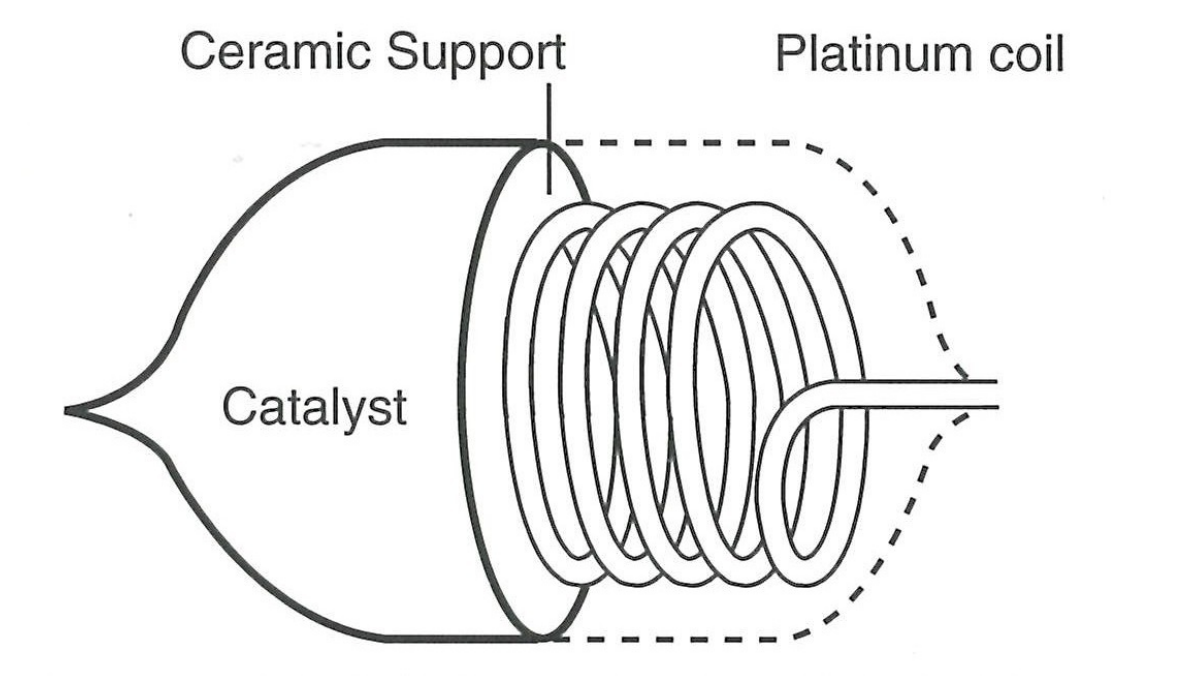
\includegraphics[scale=0.4, center]{catalytic.png}
    \caption[Structuur katalytische gassensor]{Interne structuur van een katalytische verbrandingsgassensor \autocite{gastec2016}}
    \label{fig:catalytic}
\end{figure}


\subsection{Elektrochemische gassensoren}
\label{subsec:elektrochemische}

Elektrochemische gassensoren gebruiken oxidatiereductiereacties om de gasconcentratie te meten. Wanneer een specifiek gas met het membraan (zie figuur~\ref{fig:elektrochemical}) in aanraking komt wordt het verdeeld in de elektrolyt. Deze elektrolyt kan van vast of vloeibaar materiaal zijn gemaakt. Wanneer de moleculen vervolgens in aanraking komen met de elektrode ondergaan deze een oxidatieve reactie. In deze reactie komen ionen en elektronen vrij. Zo kan er via een stroommetingssysteem worden bepaald hoeveel stroom er tussen de twee elektroden loopt (sensing- en counter elektrode in figuur~\ref{fig:elektrochemical}) \autocite{Stetter2008}.

Zo wordt de hoeveelheid gas vervolgens bepaald via de Coulomb-analyse. In deze analyse wordt de hoeveelheid gas bepaald op basis van de wet van Faraday \autocite{gvda2023}.

Deze soort gassensor kan een grote waaier aan gassen detecteren en heeft een hoge gevoeligheid \autocite{review2014}. Maar deze sensoren hebben een korte levensduur en hebben dus regelmatig nood aan onderhoud, waardoor ze niet geschikt zouden zijn als duurzame gassensor voor in een veestal.

\begin{figure}[h]
    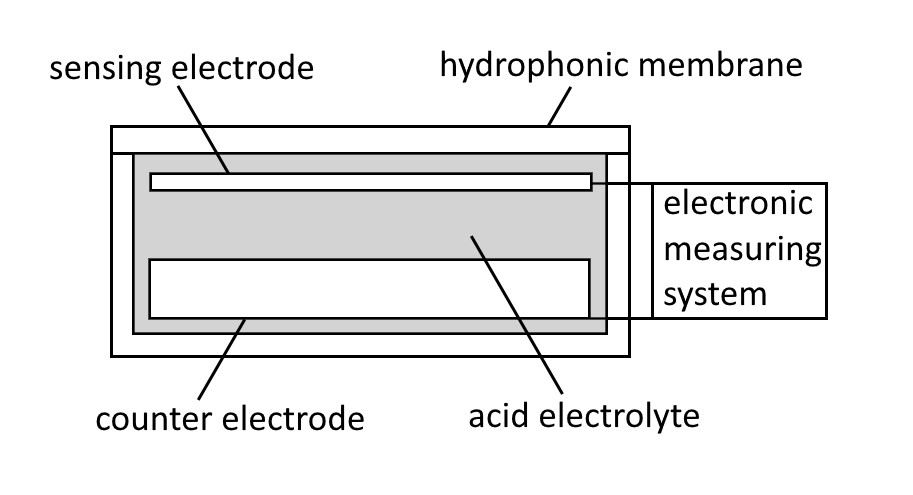
\includegraphics[scale=0.4, center]{elektrochemical.png}
    \caption[Structuur elektrochemisch gassensor]{Interne structuur van een elektrochemische gassensor \autocite{MajderLopatka2018}}
    \label{fig:elektrochemical}
\end{figure}



\subsection{Infrarood gassensoren}
\label{subsec:infrarood}

Een andere veelgebruikt gassensor is de infrarood gassensor (zie figuur~\ref{fig:infrarood}). Deze bestaat uit een lichtbron, een meetkamer en een detector. In deze lichtbron is ook een filter aanwezig. Deze filter is in staat om specifieke golflengtes van infrarood licht te selecteren.

Zo maakt de infrarood gassensor gebruik van het feit dat gasmoleculen in staat zijn om infrarode lichtstralen absorberen. Zo heeft ieder soort gas een eigen specifieke golflengte die wordt geabsorbeerd \autocite{li2010infrared}.

Wanneer de verzonden infraroodstralen de infraroodsensor verzwakt bereiken kan de gasconcentratie worden berekend. Dit gebeurt op basis van het verschil in de bereikte hoeveelheden infraroodstraling. Hoe meer gas er is, hoe minder infraroodstralen de sensor bereiken en omgekeerd \autocite{Senseair2018}. Wat betreft nauwkeurigheid en gevoeligheid is de infrarood gassensor superieur aan de andere soorten, en ook heeft deze soort sensor een langere levensuur dan de rest. Maar een infraroodsensor is wel een stuk duurder dan andere gassensoren. Ook kampt het met het probleem dat niet alle gassen infrarood licht kunnen absorberen, zoals bijvoorbeeld stikstof (N\textsubscript{2}) of waterstof (H\textsubscript{2}) \autocite{review2014}. Deze gassen kunnen dus niet worden gemeten.

\begin{figure}[h]
    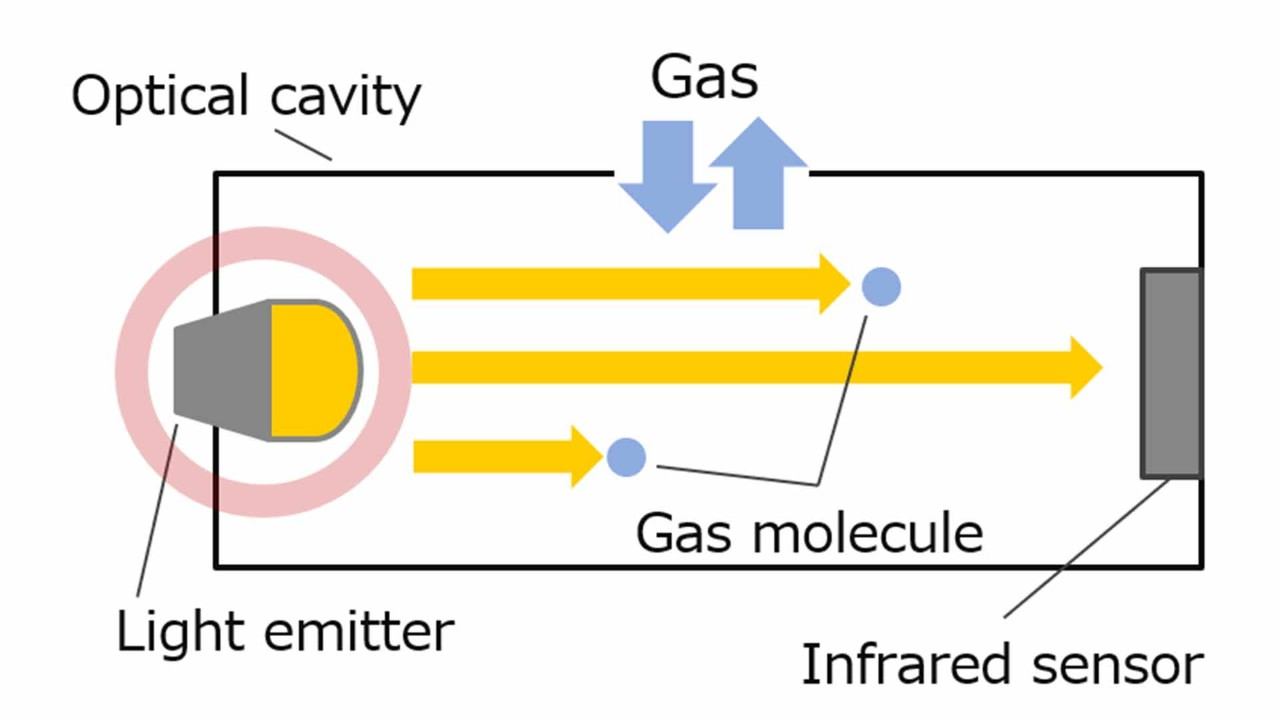
\includegraphics[scale=0.15, center]{infrarood.jpeg}
    \caption[Structuur infrarood gassensor]{Interne structuur van een infrarood gassensor \autocite{Senseair2018}}
    \label{fig:infrarood}
\end{figure}


\subsection{Halfgeleider gassensoren}
\label{subsec:MOS}

Volgens \textcite{wiki2022} is een halfgeleider een stof die op vlak van elektrische geleiding het midden houdt tussen goede geleiders en goede isolators. De halfgeleider die het meest wordt gebruikt bij gassensoren is tindioxide (SnO\textsubscript{2}) samen met een laag siliconen \autocite{Nikolic2020}. Wanneer het halfgeleidermateriaal in contact komt met een gasmolecule waarvoor het gevoelig is, treden er chemische reacties op aan het oppervlak van het materiaal. Deze reacties leiden tot veranderingen in de elektrische weerstand van het halfgeleidermateriaal. Het meetcircuit van de sensor detecteert deze verandering en zet deze om in een meetbare elektrische signaaluitgang \autocite{review2014}. Deze soort gassensoren hebben een hoge gevoeligheid, zijn goedkoop en kunnen en breed scala aan gassen detecteren. Het grootste nadeel van halfgeleider gassensoren is dat ze ook gevoelig zijn voor omgevingsfactoren zoals temperatuur en luchtvochtigheid, die de resultaten sterk kunnen beïnvloeden. Ook leiden ze aan kruisgevoeligheid, wat betekent dat ze kunnen ook reageren op andere gassen dan het doelgas, wat kan leiden tot vals-positieve resultaten.


\begin{figure}[h]
    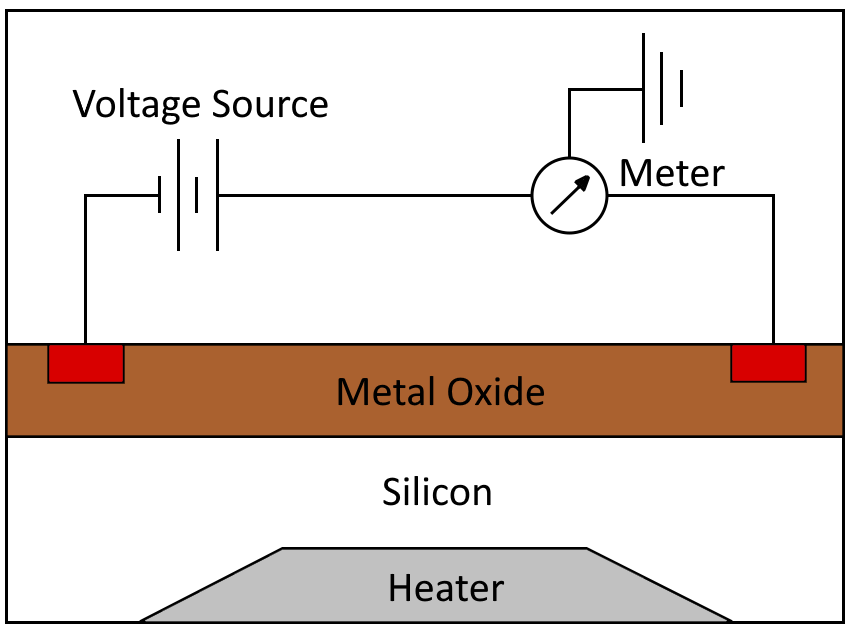
\includegraphics[scale=0.2, center]{halfgeleider.png}
    \caption[Structuur halfgeleider gassensor]{Interne structuur van een halfgeleider gassensor \autocite{review2014}}
    \label{fig:halfgeleider}
\end{figure}

\pagebreak

\section{Gebruikte hardware in de test set-up}
\label{sec:hardware}


\subsection{De MQ-gassensoren}%
\label{subsec:werking-MQ}

De MQ-gassensor is dus een gassensor van het type halfgeleider, ze kost twee tot vijf euro en kan gemakkelijk worden gebruikt via een microcontroller zoals Arduino. Het is belangrijk op te merken dat de MQ-gassensor meerdere gassen kan detecteren, maar deze niet afzonderlijk kan identificeren. De sensor geeft dus een enkele waarde terug.
De MQ-sensor heeft een voeding van 5V nodig \autocite{akp2023}, en omdat deze sensor via verwarming te werk gaat is deze beschermt met 2 lagen fijn roestvrij stalen gaas. Dit beschermende gaas zorgt ervoor dat het verwarmingselement in de sensor geen explosies veroorzaakt wanneer het in aanraking komt met een brandbaar gas.


\begin{figure}[h]
    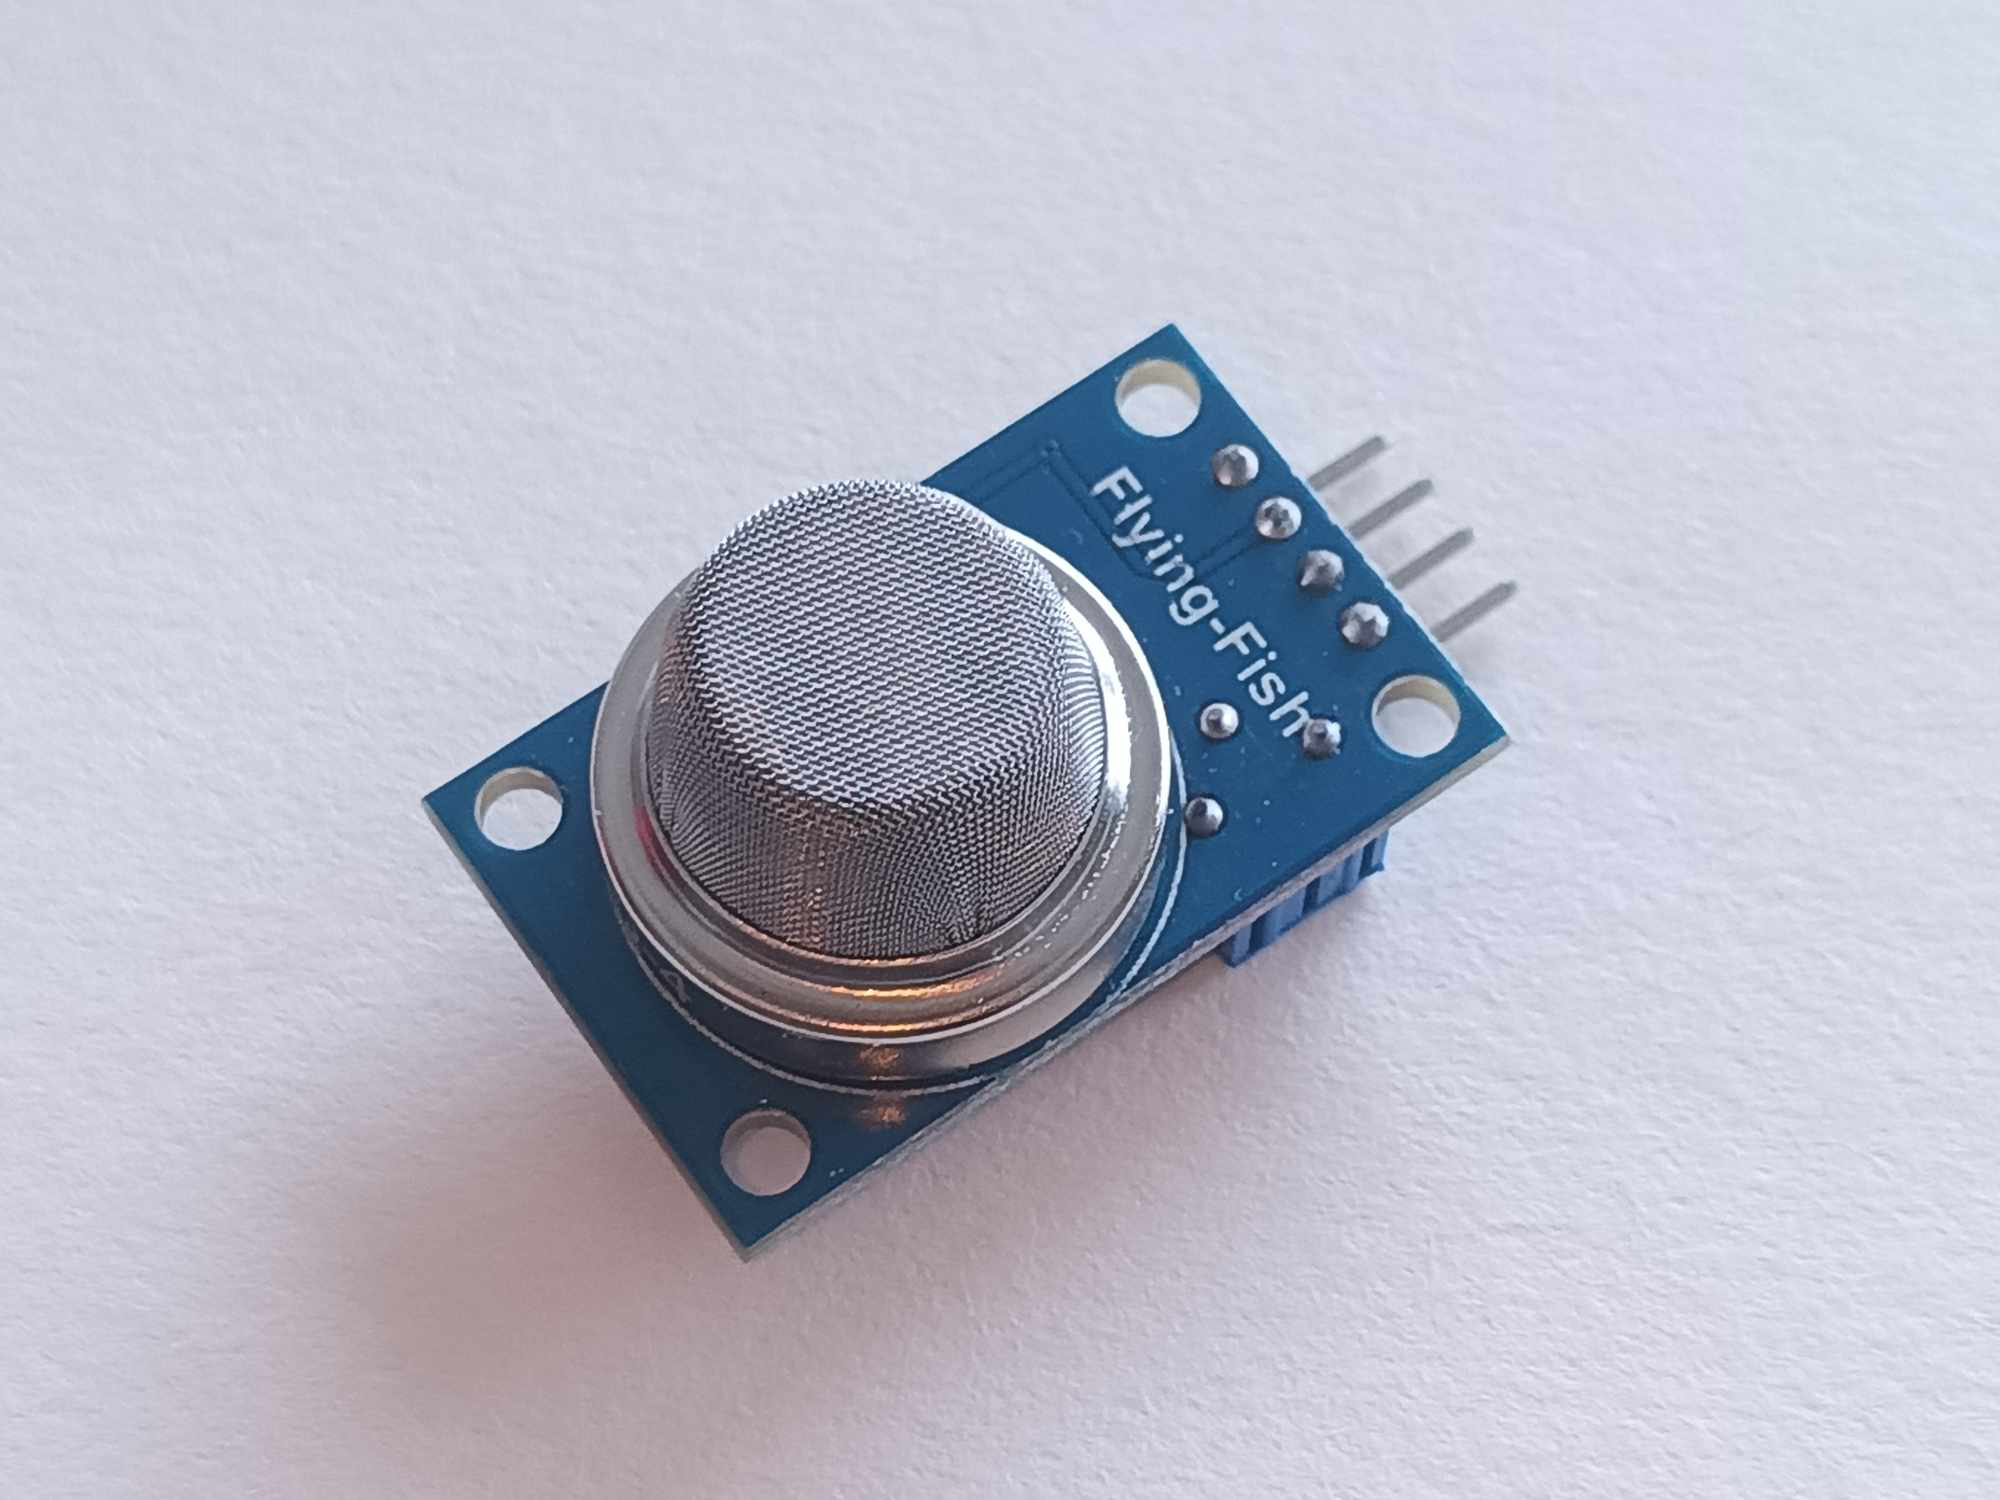
\includegraphics[scale=0.12, center]{mq.png}
    \caption[MQ-gassensor]{MQ-gassensor (links) en zijn interne structuur (rechts)}
    \label{fig:mq}
\end{figure}


De interne structuur van de sensor bestaat uit zes pinnen die verbonden zijn met een centraal sensorelement. De twee middelste pinnen zijn verantwoordelijk voor het verwarmen van het sensorelement, en de vier andere pinnen detecteren kleine variaties in de stroom die door het element gaat. Dit sensorelement bestaat uit keramiek op aluminiumoxidebasis (Al\textsubscript{2}O\textsubscript{3}), gecoat met een laag tindioxide (SnO\textsubscript{2}).


\begin{figure}[h]
    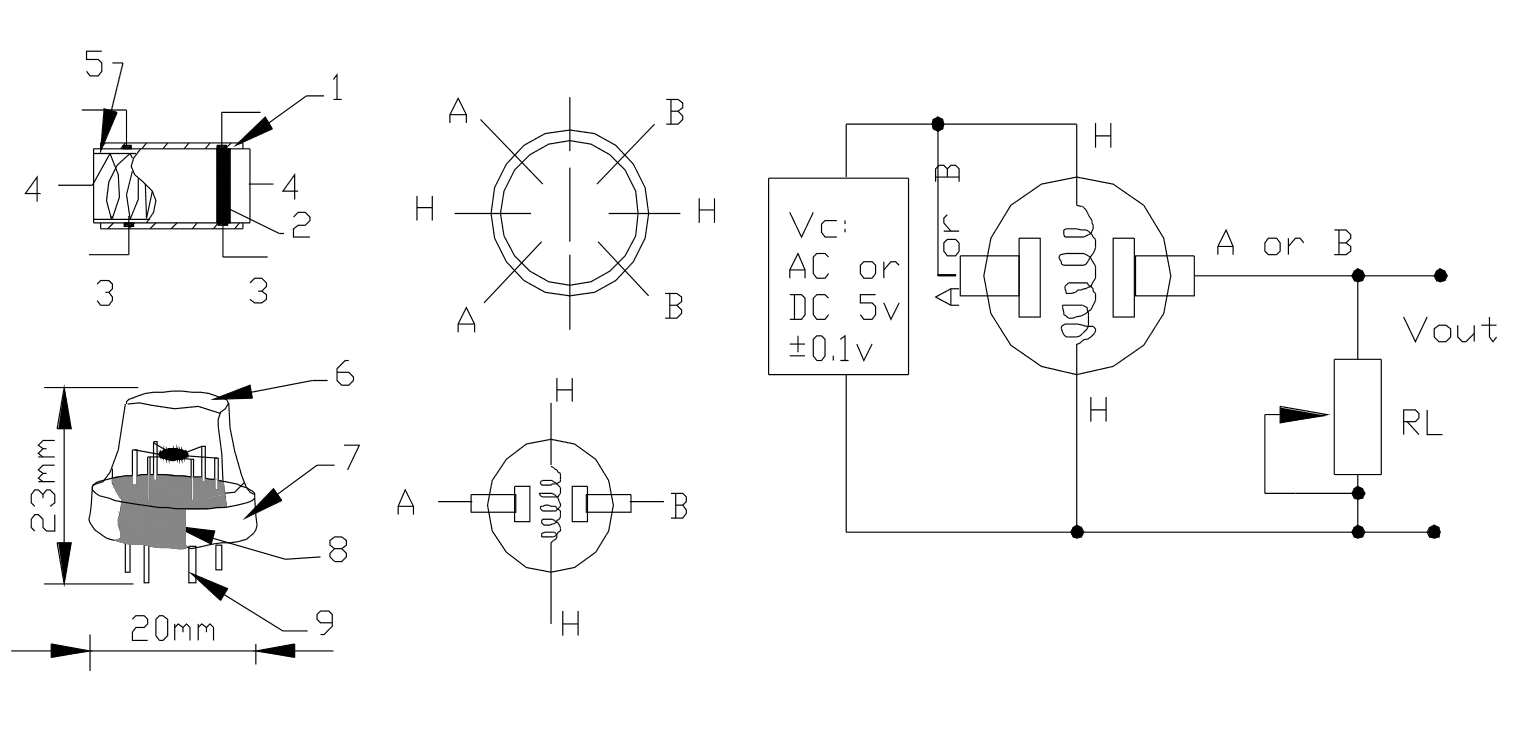
\includegraphics[scale=0.3, center]{mq_configuratie.png}
    \caption[Schema MQ-gassensor]{Schema van de structuur van een MQ-gassensor \autocite{mq4}}
    \label{fig:mq_configuratie}
\end{figure}

Wanneer deze laag SnO\textsubscript{2} wordt verwarmd blijven zuurstofmoleculen aan het oppervlak vast hangen door adsorptie. Hierdoor wordt een depletielaag gevormd, dit is een laag waar geen transport mogelijk is en dus een elektrisch isolerende laag wordt gevormd \autocite{dr2016}. Gevolglijk heeft de SnO\textsubscript{2} een hoge weerstand, waardoor de elektrische stroom wordt geblokkeerd.

Wanneer de omgeving echter andere gassen bevat kunnen deze de zuurstoflaag reduceren door middel van reductie. Als resultaat neemt de depletielaag af in dichtheid en komen er elektronen vrij in het SnO\textsubscript{2}-materiaal. Zo verminderd de weerstand en verhoogt de elektrische stroom.

Een belangrijk detail bij het gebruiken van de MQ-sensor is de voorverwarming. Doordat de sensor een lange tijd in opslag heeft gelegen verliest hij zijn nauwkeurigheid, daarom is het noodzakelijk om hem 24-48 uur te laten voorverwarmen. Hierna heeft de sensor bij iedere sessie slechts 5-10 minuten nodig om zich te stabiliseren \autocite{Sakayo2019}.

Er zijn veel verschillende soorten MQ-sensoren die elk gespecialiseerd zijn in verschillende gassen, volgens het onderzoek van \textcite{Khodadadi2001} kan de gevoeligheid voor methaan (CH\textsubscript{4}) vergroot worden door platina toe te voegen aan de SnO\textsubscript{2}. Ook kan door een toevoeging van K\textsubscript{2}O de gevoeligheid voor koolstofmonoxide (CO) worden vergroot. En op dezelfde manier kan Na\textsubscript{2}O ervoor zorgen dat de sensor minder gevoelig wordt voor CO\textsubscript{2}. Zo heeft iedere MQ-sensor kleine aanpassingen in het sensor element wat ze gevoelig maakt voor specifieke gassen.

De MQ-sensoren die gekozen zijn voor dit onderzoek zijn de MQ-4, MQ-7 en MQ-135. De MQ-4 sensor is gevoelig voor methaan (CH\textsubscript{4}) en LPG (Liquified Petroleum Gas). De MQ-7 biedt een specialisatie in koolstofmonoxide (CO) en waterstof (H\textsubscript{2}). Tenslotte is de MQ-135 een sensor die wordt gebruikt om de algemene luchtkwaliteit te meten, dit gebeurt vooral aan de hand van de gassen CO\textsubscript{2}, NH\textsubscript{4} en CO \autocite{RC2022}.

In dit onderzoek is er voor de MQ-4 en en MQ-135 sensor gewerkt met een module, dit betekent dat de sensor al op een vooraf gemaakte printplaat is bevestigd. Deze modules hebben geen zes maar vier pinnen: spanning, grond, digitale- en analoge uitgang. Het voordeel van deze modules is dat deze gemakkelijker te gebruiken zijn dan de naakte sensoren, maar het nadeel is dat de belastingsweerstand op deze modules gelijk is aan 1k$\Omega$. In de datasheets van deze sensoren (\autocite{mq135}, \autocite{mq4}) staat dat er voor optimale resultaten de aanbevolen belastingsweerstand 20k$\Omega$ is. 1 k$\Omega$ valt hier dus ver onder dus het is belangrijk hier rekening mee te houden als de ppm wordt berekend in de berekeningen (\ref{sec:hoe-luchtsamenstelling meten}).


\subsection{DHT22}%
\label{subsec:dht22}

Naast de MQ-sensoren zal ook een DHT22 sensor worden geïntegreerd in de test set-up. De DHT22 sensor meet temperatuur en luchtvochtigheid. Deze waarden kunnen van pas komen bij het optimaliseren van de resultaten van de MQ-sensoren, aangezien deze sensoren gevoelig zijn voor omgevingsfactoren zoals temperatuur en luchtvochtigheid.

In sectie~\ref{sec:temp-en-hum} zal worden berekend hoe de waarde van de MQ-sensor kan worden gecorrigeerd aan de hand van de temperatuur, de luchtvochtigheid en de info van de datasheet.

\begin{figure}[h]
    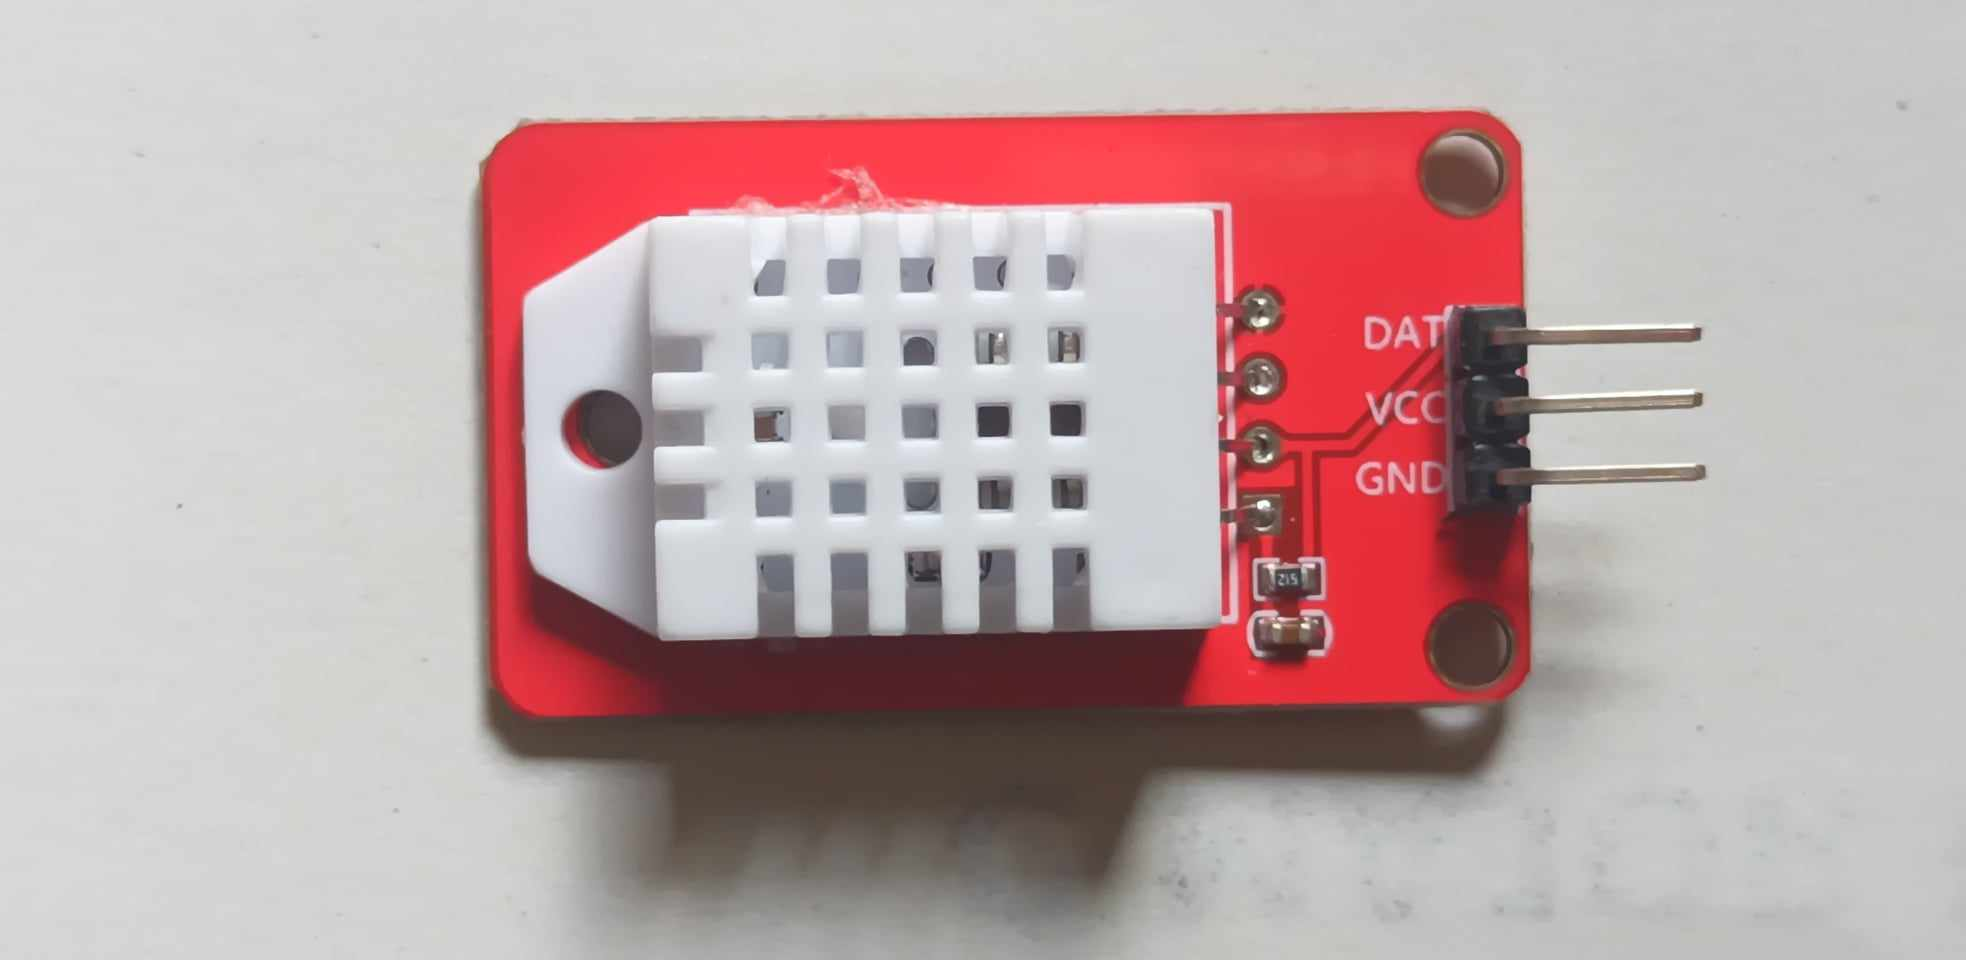
\includegraphics[scale=0.1, center]{dht22.jpg}
    \caption[DHT22 sensor]{De DHT22 sensor}
    \label{fig:dht22}
\end{figure}


\subsection{Arduino Mega 2560 Microcontroller}%
\label{subsec:arduino}

Voor dit onderzoek werd de Arduino Mega 2560 gekozen als microcontroller. De Arduino Mega 2560 is iets groter en krachtiger in vergelijking met de basis Arduino Uno voor een iets duurdere prijs. De Arduino Mega biedt een flashgeheugen van 256 KB, 54 I/O pins, 16 analoge input pins, een EEPROM (Electrically erasable programmable read-only memory) van 4kB en een SRAM (Static random-access memory) van 8 kB \autocite{Arduino}.

\begin{figure}[h]
    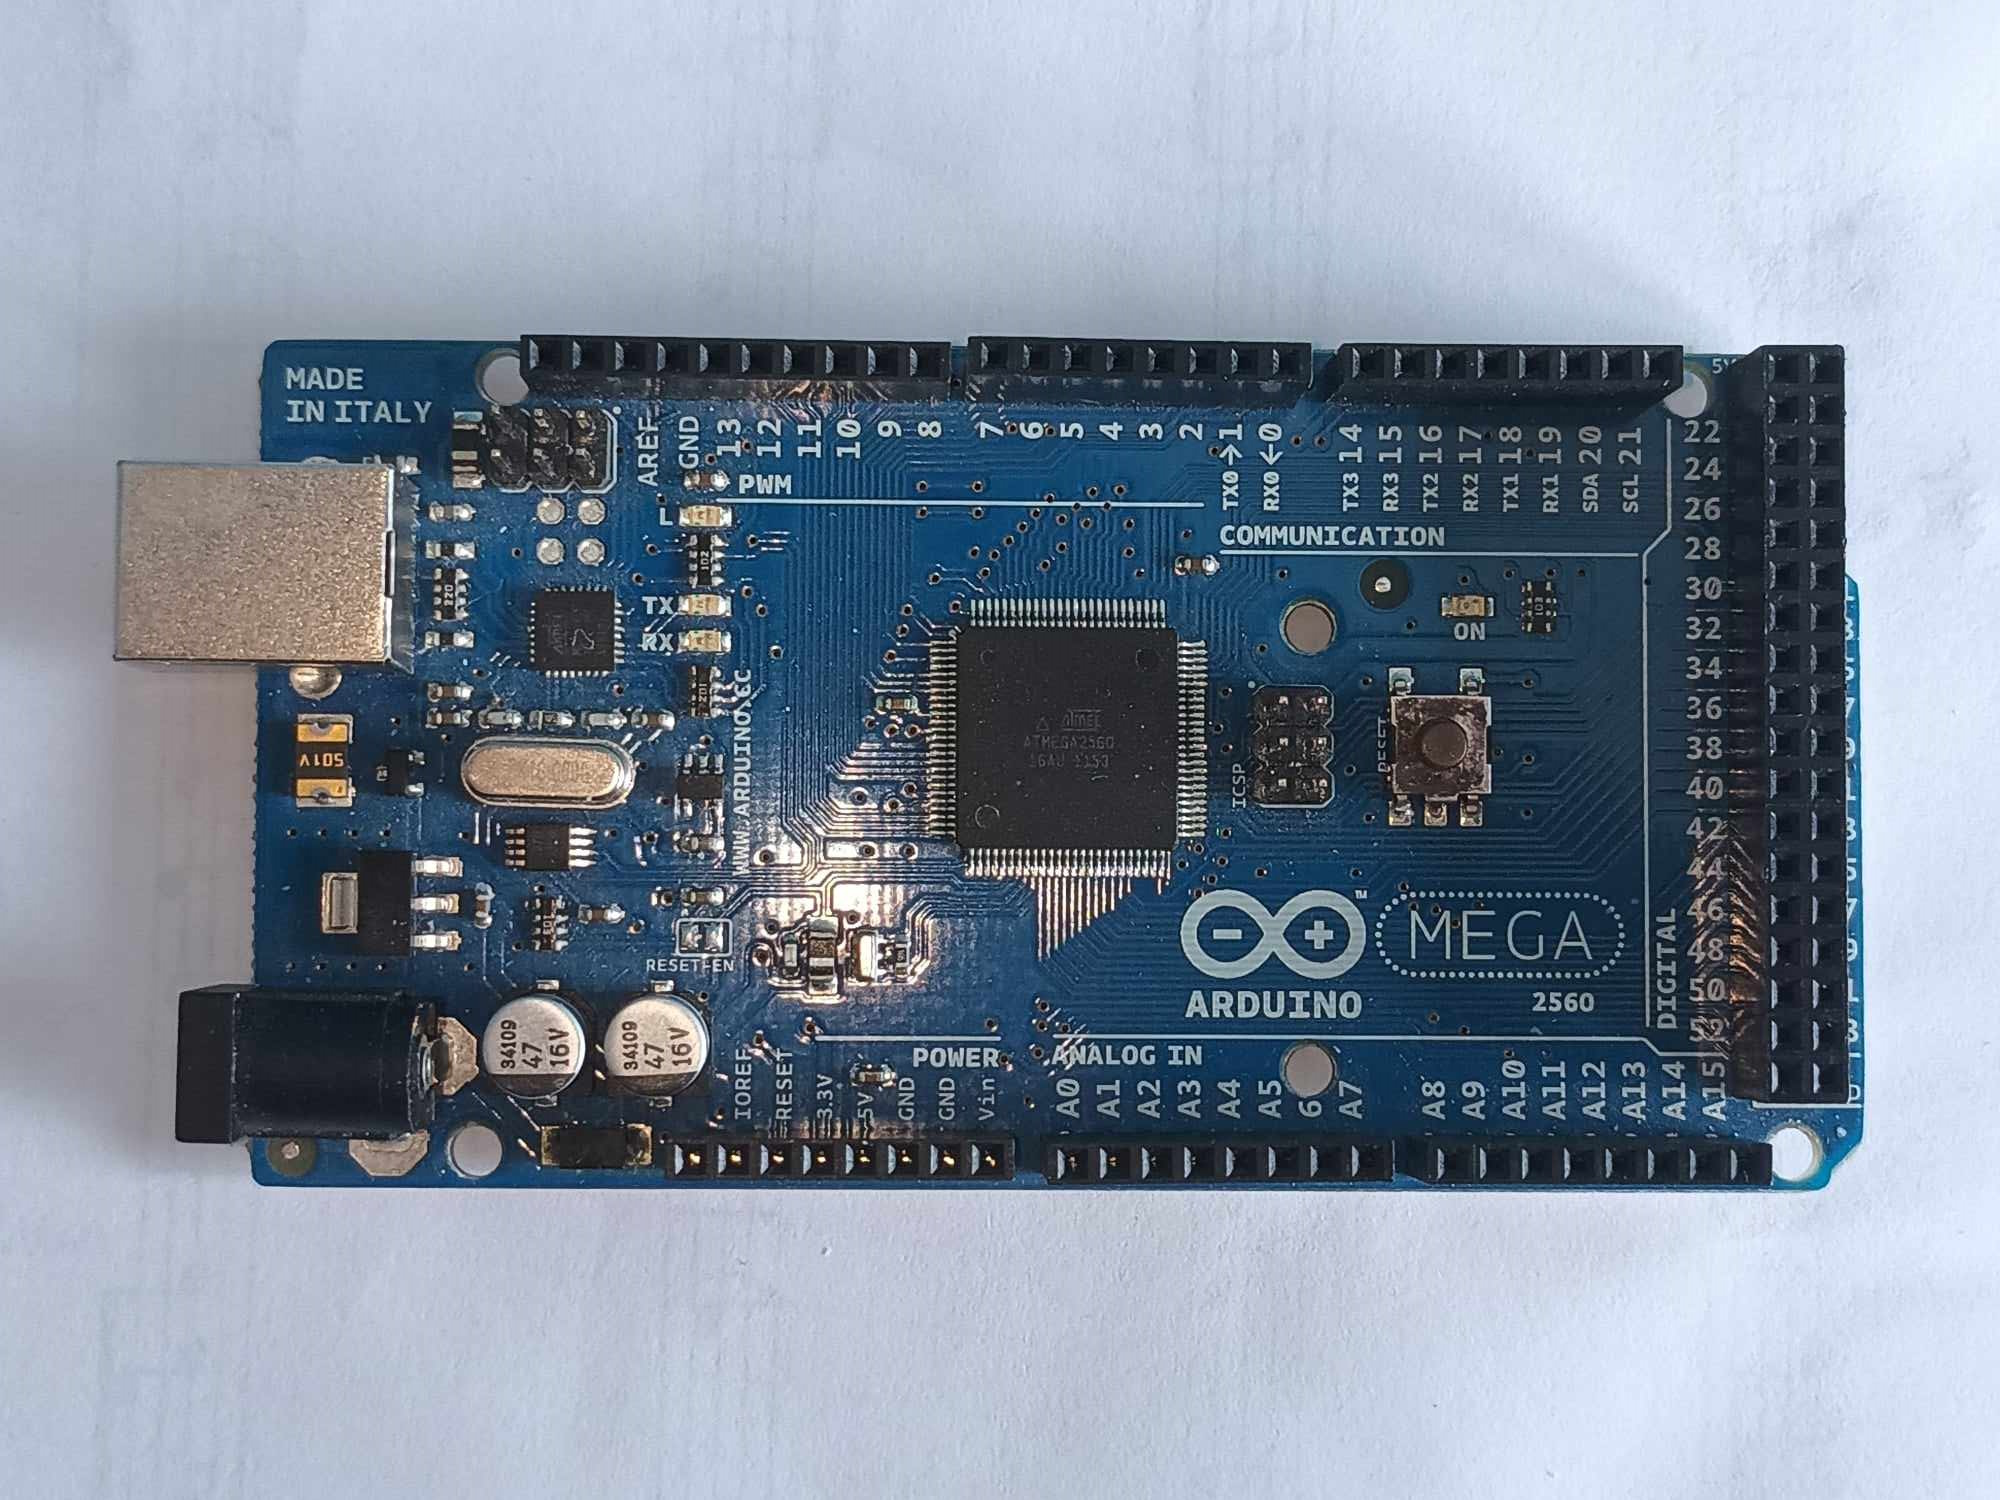
\includegraphics[scale=0.1, center]{arduino.jpg}
    \caption[Arduino Mega]{De Arduino Mega 2560}
    \label{fig:arduino}
\end{figure}


Via de Arduino IDE kan de microcontroller gemakkelijk worden geprogrammeerd om de sensoren uit te lezen en deze door te sturen naar de WiFi module.

\subsection{ESP8266-01s WiFi Module}%
\label{subsec:esp01}

De ESP8266-01s, of in het kort de ESP01, is een kleine en goedkope module die data kan versturen over een WiFi-netwerk, mits ze is aangesloten op dat netwerk. De ESP01 werkt via AT commando's, ook wel gekend als de Hayes Command Set \autocite{Bales2023}. Deze commando's worden vooral gebruikt om een ​​modem te configureren en de netwerkverbinding tot stand te brengen, maar ze zijn ook in staat data te versturen via een TCP of UDP verbinding. Zo kunnen de waarden die terug worden gegeven door de sensoren worden verzonden naar een databank en het Thingspeak platform.
Het AT-commando bestaat algemeen uit drie delen: de prefix, body en terminator. De prefix bestaat steeds uit ``AT''. De body bestaat uit de werkelijke opdracht, samen met parameters en andere gegevens. Ten slotte is er de terminator, deze is doorgaans een newline (\textbackslash r\textbackslash n) \autocite{Teltonika}.

\begin{figure}[h]
    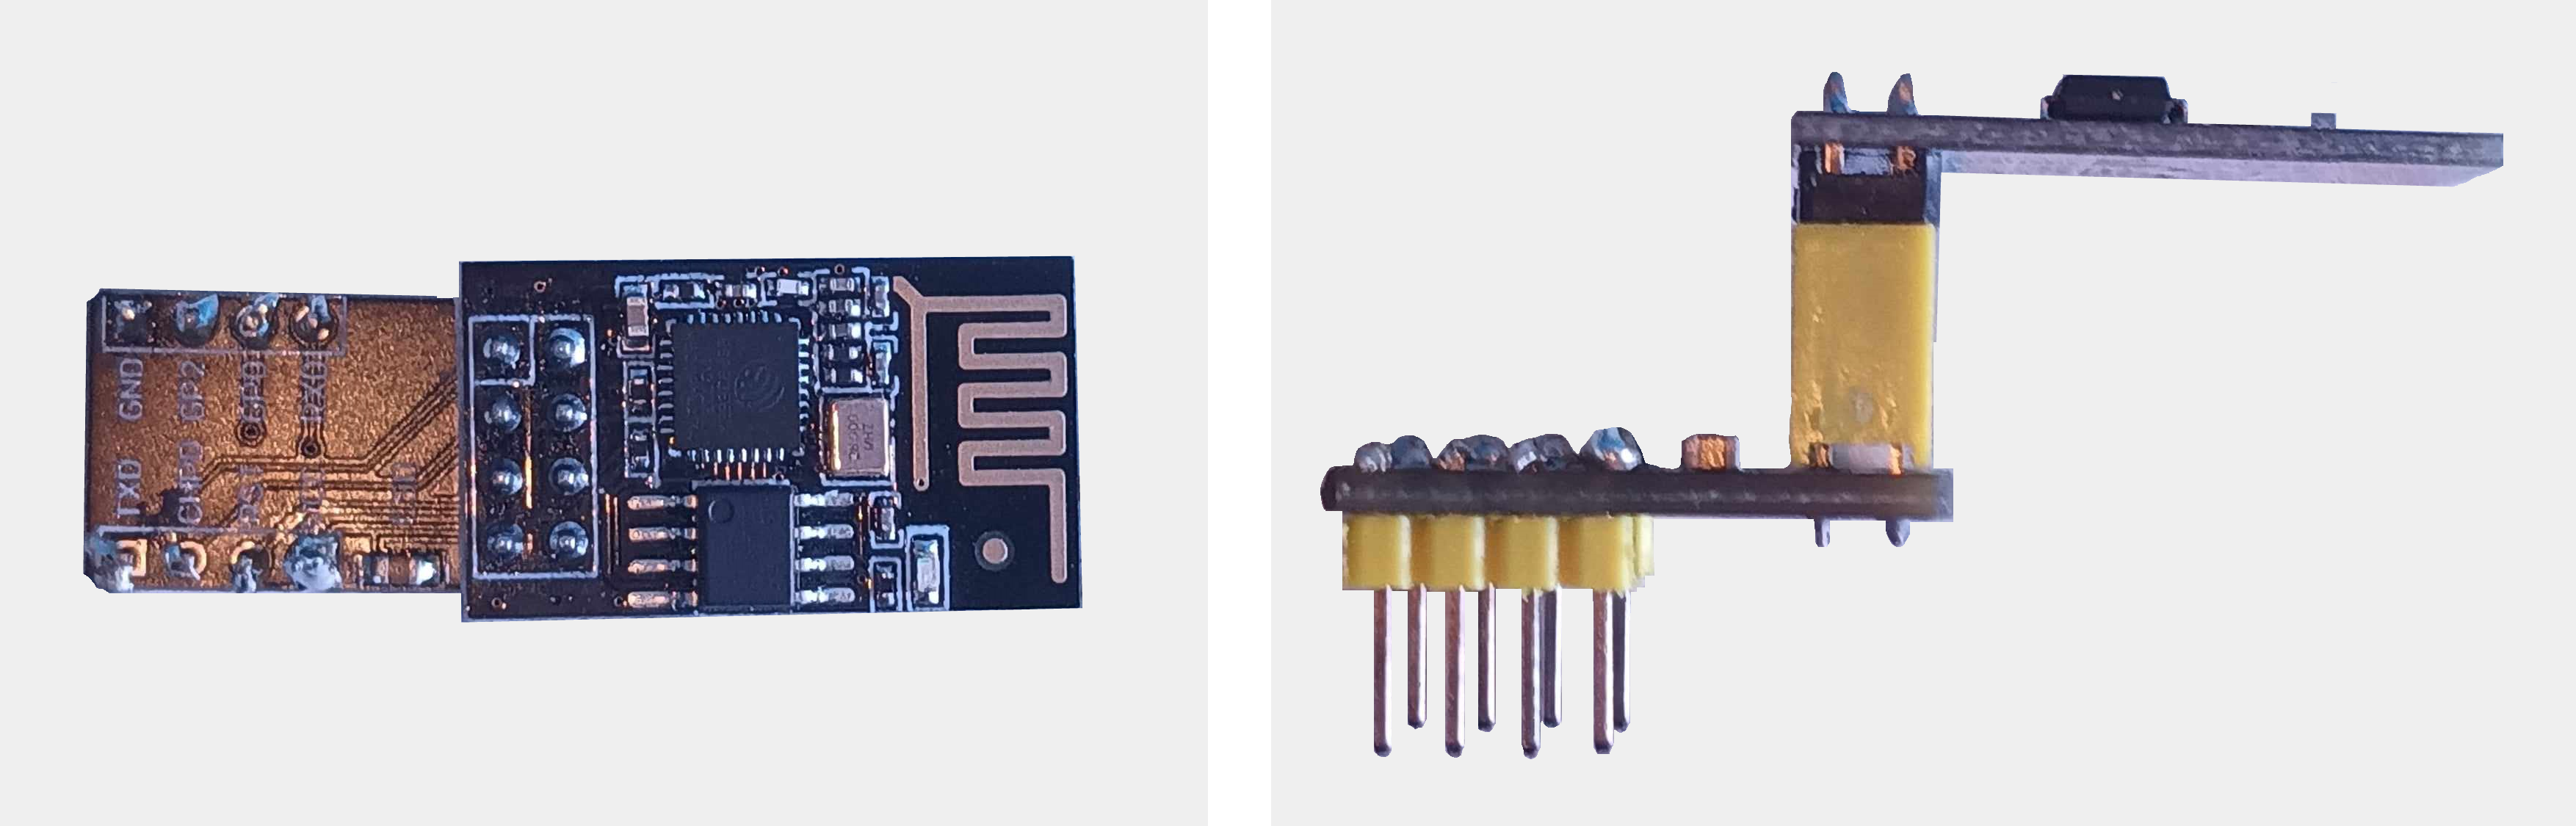
\includegraphics[scale=0.18, center]{esp.png}
    \caption[ESP01 WiFi module]{De ESP01 WiFi module met een breadboard-adapter}
    \label{fig:esp}
\end{figure}



\section{Hoe kan de luchtsamenstelling worden gemeten door MQ-sensoren?}%
\label{sec:hoe-luchtsamenstelling meten}

Een MQ-sensor geeft dus maar 1 analoge waarde terug, maar op basis van deze waarde kan een berekende schatting worden gemaakt naar de luchtsamenstelling. In de officiële datasheets van de MQ-4, -7 en -135 staan gevoeligheidscurves voor de soorten gas waar die sensor het meest gevoelig voor is (\autocite{mq4}, \autocite{mq7}, \autocite{mq135}). Zo zie je in figuur~\ref{fig:MQ135_grafiek} een voorbeeld van de gevoeligheidscurve van de MQ-135 sensor.

\begin{figure}[h]
    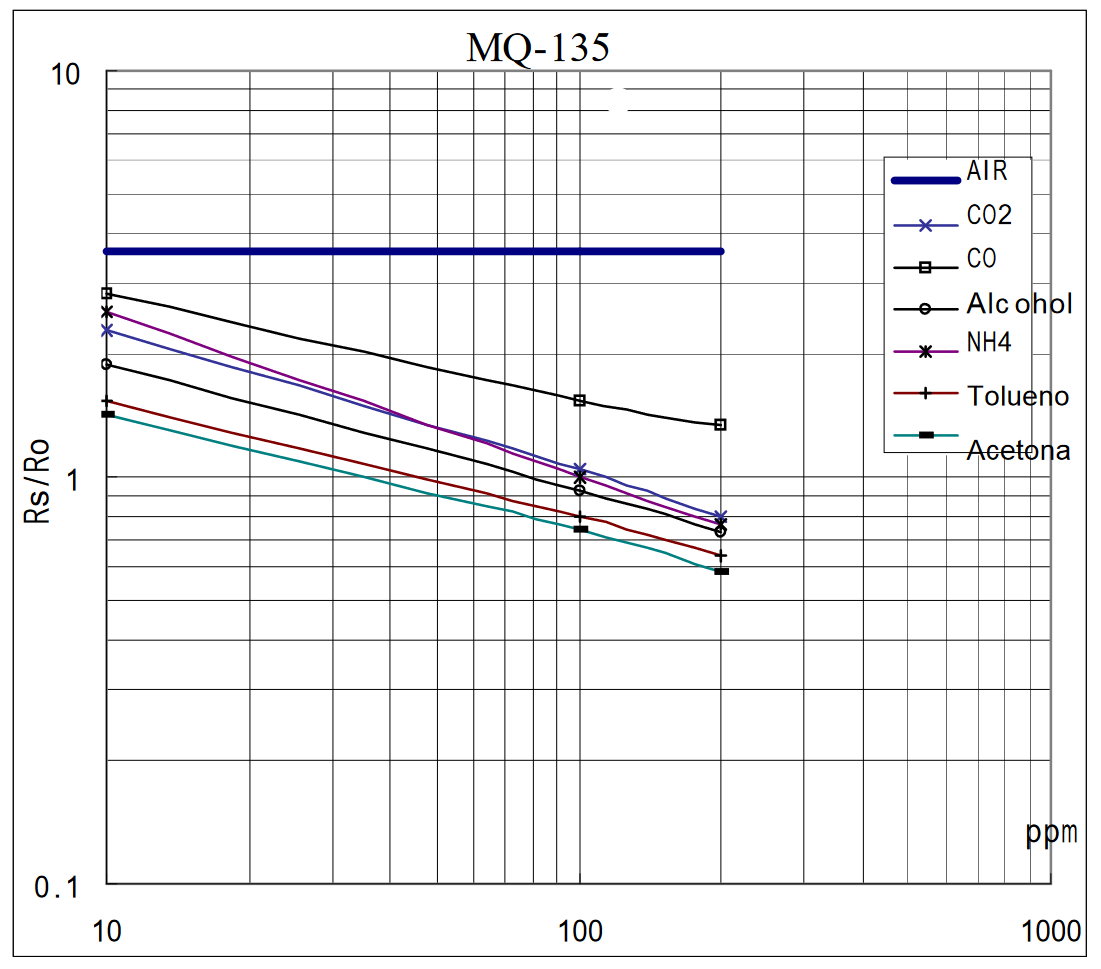
\includegraphics[scale=0.5, center]{MQ135_grafiek.png}
    \caption[Gevoeligheidscurve MQ-135]{Gevoeligheidscurve van de MQ-135 sensor \autocite{mq135}}
    \label{fig:MQ135_grafiek}
\end{figure}

\pagebreak

Via deze curves kan per type gas de PPM worden berekend, maar daarvoor moet Rs/R\textsubscript{0} zijn gekend. De volgende berekeningen tonen hoe Rs en R0 kunnen worden berekend, waarmee vervolgens een analoge waarde kan worden omgezet naar PPM.

Het omzetten van de analoge waarden (0-1023) die Arduino teruggeeft naar spanningswaarden gaat als volgt:
\begin{equation}
    Vout = \frac{analoge\_waarde * Vcc}{max\_analoge\_waarde}
\end{equation}
Met Vcc = voedingsspanning in het circuit (= 5V) en max\_analoge\_waarde = 1023.

Daarna moet Rs worden gevonden, we beginnen met de wet van Ohm (met U = spanning in V, I = stroomsterkte in A en R = weerstand in $\Omega$):
\begin{equation}
    U = I * R
\end{equation}
\begin{equation}
    I = \frac{U}{R}
\end{equation}
\begin{equation}
    I = \frac{Vcc}{Rs+Rl}
\end{equation}
Met Rl = belastingsweerstand van het circuit en Rs = weerstand van de sensor

Terug naar Ohm:
\begin{equation}
    U = I * R
\end{equation}
\begin{equation}
    VRL = \frac{Vcc}{Rs + Rl} * Rl
\end{equation}
Met VRL = voltage reference low \textbf{(= Vout)}
\begin{equation}
    Rs = \frac{Vcc * Rl}{VRL} - Rl
\end{equation}
Nu de formule voor Rs te berekenen gekend is, moeten we kijken naar R0. R0 is de weerstand van de sensor in schone lucht. Op de gevoeligheidscurve (\ref{fig:MQ135_grafiek}) is te zien hoe Rs/R\textsubscript{0} een constante is voor schone lucht. Via software zoals WebPlotDigitizer \autocite{Rohatgi2024} kan de waarde van deze constante worden opgehaald. Voor de MQ-135 is deze waarde 3,6.

Dus:
\begin{equation}
    \frac{Rs}{R_0}(voor\ schone\ lucht) = 3,6
\end{equation}
\begin{equation}
    R_0 = \frac{Rs}{3,6}
\end{equation}
Om de sensor te kalibreren moet dus de R\textsubscript{0} waarde worden berekend. Het is dus zeer belangrijk dat de sensor 24-48 heeft voorverwarmd en dat de kalibratie in schone lucht gebeurt, anders kan de R\textsubscript{0} waarde afwijken en zullen de lezingen incorrect zijn.

Om de ppm waarde te berekenen kijken we opnieuw naar de gevoeligheidscurves (\ref{fig:MQ135_grafiek}). Deze curves lijken lineair te dalen, maar deze grafiek is dubbellogaritmisch. Volgens \textcite{loglog2024} is de vergelijking voor een lineaire curve in een dubbellogaritmische weergave de volgende:
\begin{equation}
    F(x) = x^{m} * 10^{b}
\end{equation}
Met m = gradiënt (de helling) en b = het snijpunt met de Y-as.

Volgens de MQ-135 grafiek is dit dan:
\begin{equation}
    \label{eq:grafiek}
    \frac{Rs}{R_0} = ppm^{m} * 10^{b}
\end{equation}
\begin{equation}
    \log_{10} (\frac{Rs}{R_0}) = m * \log_{10} (ppm) + b
\end{equation}
Om de ppm van een specifiek gas te berekenen hebben we $m$ en $b$ nodig. Hiervoor nemen we 2 punten op de curve van het gewenste gas waarvoor de ppm moet worden berekend (\ref{fig:MQ135_grafiek}), dit kan opnieuw worden gedaan met WebPlotDigitizer \autocite{Rohatgi2024}. Deze punten zullen we $x1,\ x2,\ y1\ en\ y2$ noemen:
\begin{eqnarray}
    \begin{cases}
        \log_{10} (y1) = m * \log_{10} (x1) + b\\
        \log_{10} (y2) = m * \log_{10} (x2) + b\\
    \end{cases}
\end{eqnarray}
\begin{eqnarray}
    \begin{cases}
        m = \frac{log_{10} (y2) - log_{10} (y1)}{log_{10} (x2) - log_{10} (x1)} \\
        b = log_{10} (y1) - m * log_{10} (x1)\\
    \end{cases}
\end{eqnarray}
Nu dat $m$ en $b$ zijn gekend kan de ppm worden berekend via vergelijking~\ref{eq:grafiek}:
\begin{equation}
    ppm = \Big(\frac{Rs}{R_0 * 10^{b}}\Big)^{\frac{1}{m}}
\end{equation}

De volgende bronnen werden geraadpleegd bij het berekenen van deze waarden: \autocite{ohm2024}, \autocite{Cornelius2022}, \autocite{KumarSai2019}, \autocite{Dorcea2018}, \autocite{jaycon2023}, \autocite{Kalra2016}, \autocite{RapidTables}, \autocite{Ibrahim2022}, \autocite{Gironi2014} en \autocite{Gironi2017}.



\section{Hoe gaat een sensor met een warmte-koelcyclus te werk?}%
\label{sec:warmte-koelcyclus}


Volgens de officiële datasheet van de MQ-7 sensor is het werkingsprincipe voor deze sensor anders dan de MQ-4 en -135 sensoren. Voor optimale resultaten moet er namelijk gebruik worden gemaakt van een warmte-koelcyclus. In deze cyclus wordt doorheen twee fases gegaan, een fase van lage verwarming en een fase van hoge verwarming. Tijdens de lage temperatuurfase wordt gedurende 90 seconden 1,4V naar de sensor verzonden. In deze fase wordt gas geabsorbeerd op de plaat, op het einde kan de waarde worden afgelezen. Tijdens de hoge temperatuurfase wordt gedurende 60 seconden 5V naar de sensor verzonden. In deze fase verdampen geabsorbeerde gassen van de sensorplaat, waardoor deze wordt gereinigd voor de volgende meting \autocite{Kobbekaduwa2021}. Een duidelijk voorbeeld hiervan is te zien in de figuur (\ref{fig:heat_cool_datasheet}) van de datasheet

\begin{figure}[h!]
    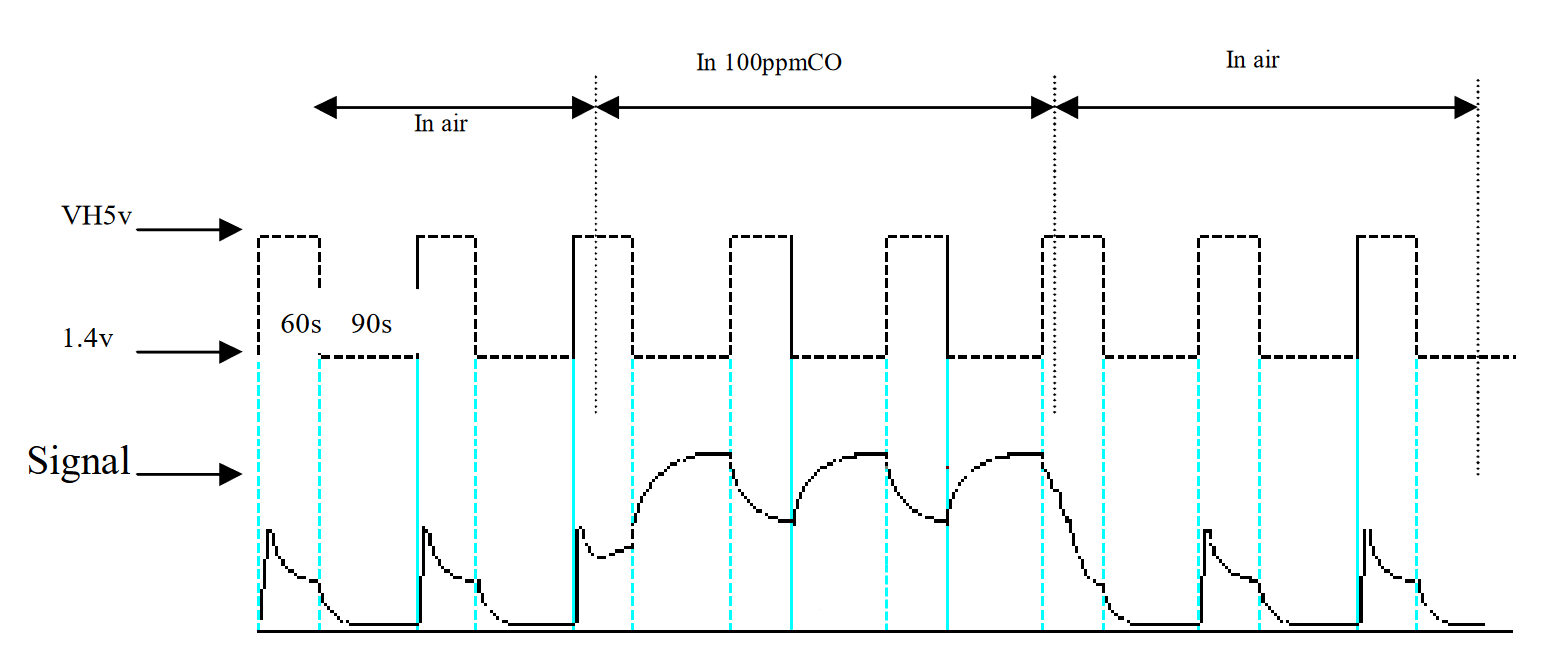
\includegraphics[scale=0.3, center]{heat_cool_datasheet.png}
    \caption[Warmte-koelcyclus MQ-7]{Een voorbeeld van de warmte-koelcyclus in de datasheet van de MQ-7 \autocite{mq7}}
    \label{fig:heat_cool_datasheet}
\end{figure}

In de studie van \textcite{Kobbekaduwa2021} is te zien hoe deze warmte-koelcyclus kan worden geïmplementeerd. De benodigde materialen (naast de MQ-7 en Arduino) zijn twee weerstanden van 10$k\Omega$ en een MOSFET transistor van het type IRF2807.


\section{Hoe kunnen de temperatuur en luchtvochtigheid tot nauwkeurigere resultaten leiden?}
\label{sec:temp-en-hum}

Zoals besproken in~\ref{subsec:MOS} zijn halfgeleider gassensoren gevoelig voor omgevingsfactoren zoals temperatuur en luchtvochtigheid. Een sensor zoals de DHT22 \autocite{Liu} kan deze omgevingsfactoren meten en kan zo de resultaten van de MQ-sensoren optimaliseren.

Volgens \textcite{Kalra2016} en \textcite{Cornelius2023} kan $Rs$ worden gecorrigeerd om zo een correctere ppm te verkrijgen. In de datasheets (\autocite{mq4}, \autocite{mq7}, \autocite{mq135}) van de MQ-sensoren staan naast gevoeligheidscurves grafieken die de invloed van temperatuur en vochtigheid weergeven. Zo zie je bijvoorbeeld in figuur~\ref{fig:MQ135_grafiek2} de afhankelijkheidsgrafiek van de MQ-135 datasheet.

\begin{figure}[h]
    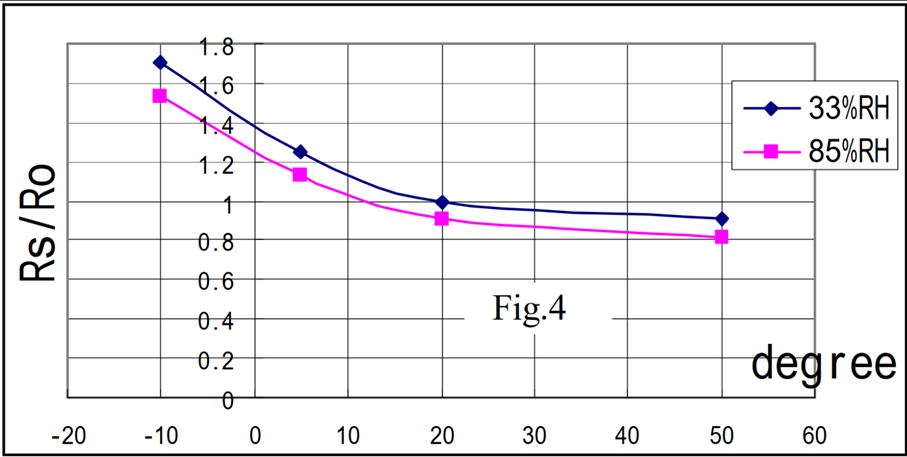
\includegraphics[scale=0.55, center]{MQ135_grafiek2.png}
    \caption[Afhankelijkheid temperatuur en luchtvochtigheid op MQ-135]{Afhankelijkheidsgrafiek van temperatuur en luchtvochtigheid op de resultaten van de MQ-135 \autocite{mq135}}
    \label{fig:MQ135_grafiek2}
\end{figure}

In de blog van software-ingenieur \textcite{Gironi20172} en in de studie van \textcite{Sukhdev2022} wordt vastgesteld dat via lineaire interpolatie de juiste correctiefactor kan worden berekent.

Aan de hand van de volgende stappen wordt duidelijk gemaakt hoe de correctiefactor kan worden berekend:

We beginnen met de afhankelijkheidsgrafiek van de datasheet (\ref{fig:MQ135_grafiek2}). Hier is te zien hoe Rs/R\textsubscript{0} kleiner wordt naarmate de temperatuur en vochtigheidsgraad stijgen. Via WebPlotDigitizer kunnen opnieuw de waarden uit deze grafieken gehaald worden \autocite{Rohatgi2024}. Hierna kan er via de \verb|polyfit| functie van Python package \verb|numpy| curve fitting worden gedaan op deze datapunten, zoals in de volgende listing:
\begin{lstlisting}[language=Python, caption={Curve fitting in Python}]
import pandas as pd
import numpy as np

mq135_humidity_33 = {'x': [ datapunten x ],
                    'y': [ datapunten y ]}
mq135_humidity_33_df = pd.DataFrame(mq135_humidity_33)

mq135_humidity_33_fit = np.polyfit(mq135_humidity_33_df['x'], mq135_humidity_33_df['y'], 2) #functie van de 2de graad

\end{lstlisting}

Als dit voor alle grafieken wordt gedaan wordt het resultaat in figuur~\ref{fig:curve_fitting_NOG_NIET} verkregen.

\begin{figure}[h]
    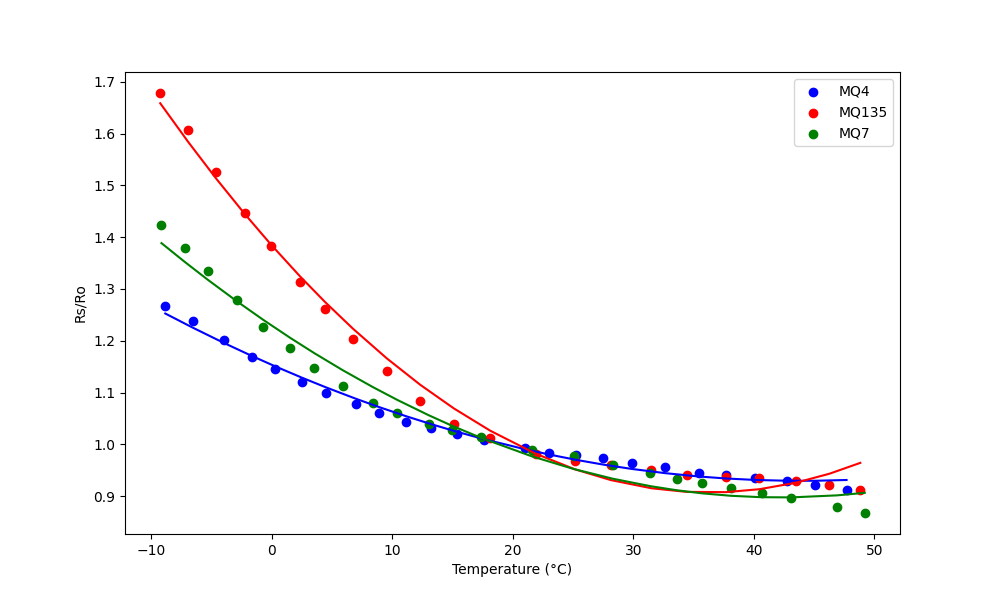
\includegraphics[scale=0.43, center]{curve_fitting_NOG_NIET.png}
    \caption[Niet optimale curve-fit op de datapunten]{Niet optimale curve-fit op de datapunten}
    \label{fig:curve_fitting_NOG_NIET}
\end{figure}

In deze grafiek is te zien hoe de curve fitting vanaf 20°C niet meer correct is, daarom zal de curve fitting worden opgesplitst. Voor de temperaturen onder 20°C zal een functie van de 2\textsubscript{de} graad worden toegepast, voor alle temperaturen hierboven zal gebruik worden gemaakt van een lineaire functie. Het resultaat is te zien in figuur~\ref{fig:curve_fitting_GOED}.

\begin{figure}[!h]
    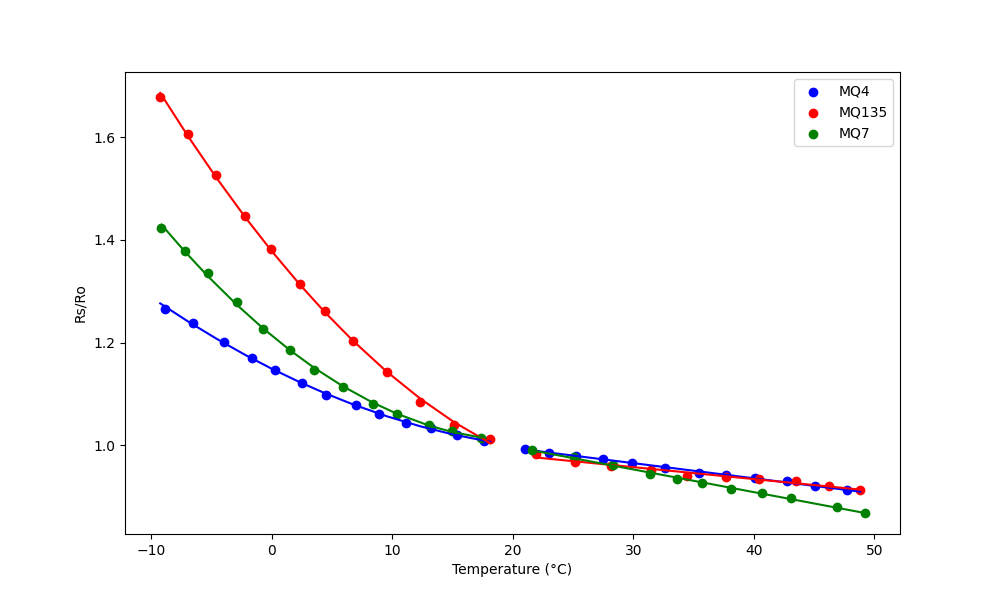
\includegraphics[scale=0.43, center]{curve_fitting_GOED.png}
    \caption[Optimale curve-fit op de datapunten]{Optimale curve-fit op de datapunten}
    \label{fig:curve_fitting_GOED}
\end{figure}

Zo zijn de functies voor de MQ-135 (\ref{fig:MQ135_grafiek2}) de volgende:

\(MQ135\_humidity\_33\_under\_20\ =\ 0.00046 * x^2 - 0.02907 * x + 1.37849\) \\
\(MQ135\_humidity\_85\_under\_20\ =\ 0.00041 * x^2 - 0.02534 * x + 1.24596\) \\
\(MQ135\_humidity\_33\_over\_20\ =\ -0.00233 * x + 1.02679\) \\
\(MQ135\_humidity\_85\_over\_20\ =\ -0.00273 * x + 0.95286\)

Nu de vergelijkingen voor alle grafieken gekend zijn kan de correctiefactor worden berekend. In het volgende voorbeeld wordt aangetoond hoe dit kan: stel dat we met de MQ-135 sensor een meting hebben gedaan waarbij de $temperatuur$ gelijk is aan $23$°C en de $vochtigheidsgraad$ gelijk is aan $55\%$. Aangezien de temperatuur boven de 20°C ligt zullen de lineaire vergelijkingen worden gebruikt.
Eerst zal Rs/R\textsubscript{0} worden berekend voor $temperatuur = 23$°C:

\begin{equation}
    F\_33(t) = -0.00233 * t + 1.02679
\end{equation}
\begin{equation}
    F\_33(23) = 0.9732
\end{equation}
En hetzelfde voor vochtigheidsgraad 85\%:
\begin{equation}
    F\_85(23) = 0.89007
\end{equation}

Als er vanuit wordt gegaan dat de luchtvochtigheidsgraad lineair afhankelijk is (wat niet zeker is aangezien er maar 2 waarden in de datasheet zijn gegeven!) kan de rechtse grafiek in figuur~\ref{fig:berekeningen} worden opgesteld, waarbij de X-as is nu luchtvochtigheid is.

Via lineaire interpolatie \autocite{lin2016} kan nu de correctiefactor voor Rs/R\textsubscript{0} worden berekend:

\begin{equation}
    y = y1 + \frac{y2 - y1}{x2 - x1}*(x - x1)
\end{equation}
\begin{equation}
    y = 0.9732 + \frac{0.89007 - 0.9732}{85 - 33}*(55 - 33)
\end{equation}
\begin{equation}
    y = 0.93802
\end{equation}

Nu is Rs/R\textsubscript{0}:
\begin{equation}
    correcte\_Rs/R_0 = \frac{Rs}{R_0} * 0.93802
\end{equation}


\begin{figure}[h]
    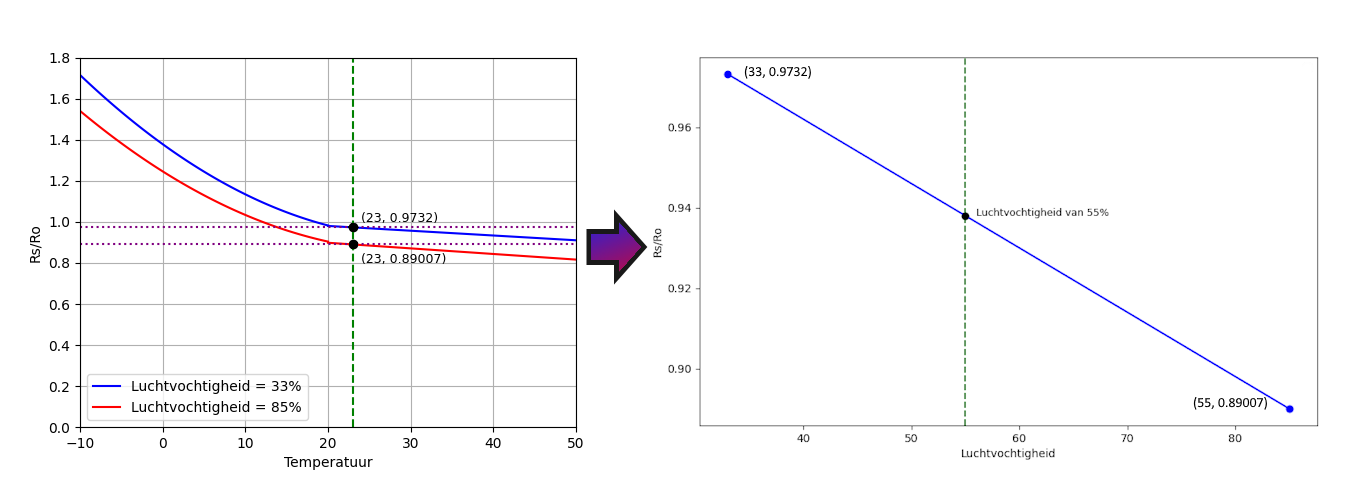
\includegraphics[scale=0.55, center]{berekeningen.png}
    \caption[Voorbeeld berekenen Rs/R0 met temperatuur = 23°C en luchtvochtigheid = 55\%]{Voorbeeld berekenen van de Rs/R0 waarden voor een temperatuur van 23°C en een luchtvochtigheid van 55\%}
    \label{fig:berekeningen}
\end{figure}


